\def\figdir{/storage/emulated/0/Documents/documents/latex/1920/Grade-8/3rd/proving-parallelograms/f}
\def\lenB{1.5in}

%\textbf{Practice Exercises}
\textbf{Problem Set}

\vspce

Find the values of $x$ and $y$ that ensure each quadrilateral is a parallelogram. 

\begin{center}

\noindent\begin{minipage}{\textwidth}
\begin{tabularx}{\textwidth}{|X|X|}
\hline
1. 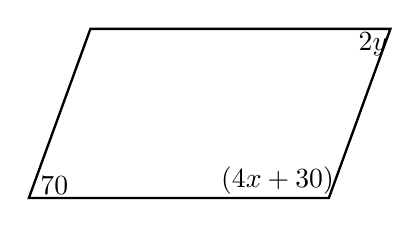
\begin{tikzpicture}

\def\len1{\lenB}

\draw[line width=0.3mm] (0,0) coordinate (a)  -- (0:\len1) coordinate (b) --++ (70:0.6*\len1) coordinate (c) -- (70:0.6*\len1) coordinate (d) -- cycle;  

\node[anchor=south east, inner sep=1pt, rotate=0, xshift=3pt, yshift=0pt] (b-label) at (b) {$ (4x+30)\degree $}; 

\node[anchor=south west, inner sep=1pt, rotate=0, xshift=3pt, yshift=0pt] (a-label) at (a) {$ 70\degree $}; 

\node[anchor=north east, inner sep=1pt, rotate=0, xshift=0pt, yshift=0pt] (c-label) at (c) {$ 2y\degree $}; 

\end{tikzpicture} 
& 
3. \begin{tikzpicture}

\def\len3{\lenB}

\draw[line width=0.3mm] (0,0) coordinate (a)  -- (0:\len3) coordinate (b) --++ (75:\len3) coordinate (c) -- (75:\len3) coordinate (d) -- cycle -- (c) (b) -- (d) ; 

\coordinate (tick1) at ($(a)!0.25!(c)$) {};

\coordinate (tick2) at ($(a)!0.75!(c)$) {};  

\tikzset{onetick/.pic={\draw[line width=0.3mm] ($(0,0)+(0, 0.06*\len3)$) -- ($(0,0)-(0, 0.06*\len3)$) ; }}

\pic[rotate=38] at (tick1) [pic type = onetick]; 

\pic[rotate=38] at (tick2) [pic type = onetick];   

\node[anchor=south west, inner sep=0pt, rotate=0, xshift=0pt, yshift=0pt] (7x-6) at ($(b)!0.75!(d)$) {$ 7x-6$};

\node[anchor=south west, inner sep=0pt, rotate=0, xshift=0pt, yshift=0pt] (4x+3) at ($(b)!0.25!(d)$) {$ 4x+3$}; 

\end{tikzpicture} \\
\hline
2. 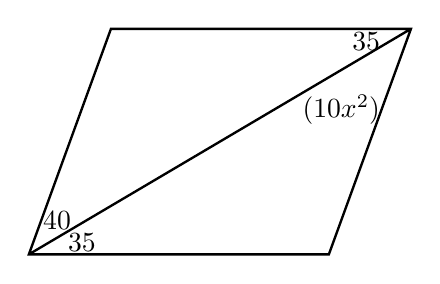
\begin{tikzpicture}

\def\len2{\lenB}

\draw[line width=0.3mm] (0,0) coordinate (a)  -- (0:\len2) coordinate (b) --++ (70:0.8*\len2) coordinate (c) -- (70:0.8*\len2) coordinate (d) -- cycle -- (c);  

\node[anchor=south west, inner sep=1pt, rotate=0, xshift=0.4em, yshift=1.8ex] (a-label) at (a) {$ 40\degree $};

\node[anchor=south west, inner sep=1pt, rotate=0, xshift=1.3em, yshift=0pt] (35-label) at (a) {$ 35\degree $}; 

\node[anchor=north east, inner sep=1pt, rotate=0, xshift=-1em, yshift=0pt] (c-label) at (c) {$ 35 \degree $}; 

\node[anchor=north east, inner sep=1pt, rotate=0, xshift=-1em, yshift=-5.3ex] (5x2-label) at (c) {$ (10x^2) \degree $}; 

\end{tikzpicture} 
& 
4. \begin{tikzpicture}

\def\len4{\lenB}

\draw[line width=0.3mm] (0,0) coordinate (a)  -- (0:\len4) coordinate (b) --++ (110:0.75*\len4) coordinate (c) -- (110:0.75*\len4) coordinate (d) -- cycle -- (c) (b) -- (d) ; 

\node[anchor=south west, inner sep=0pt, rotate=0, xshift=0pt, yshift=0pt] (9a) at ($(b)!0.25!(d)$) {$ 41$};

\node[anchor=south west, inner sep=0pt, rotate=0, xshift=0pt, yshift=0pt] (9b) at ($(b)!0.75!(d)$) {$ 41$};

\node[anchor=south east, inner sep=0pt, rotate=0, xshift=0pt, yshift=0pt] (48) at ($(a)!0.25!(c)$) {$ 36$};

\node[anchor=south east, inner sep=0pt, rotate=0, xshift=0pt, yshift=0pt] (3x2) at ($(a)!0.75!(c)$) {$ 4x^2$};

\end{tikzpicture} \\
\hline
\end{tabularx} 
\end{minipage}
\end{center} 

\newpage 

\begin{center}
\noindent\begin{minipage}{\textwidth}
\begin{tabularx}{\textwidth}{|X|X|}
\hline 
5. 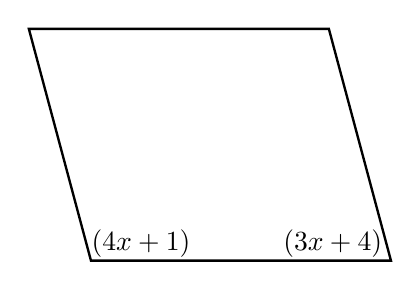
\begin{tikzpicture}

\def\len5{\lenB}

\draw[line width=0.3mm] (0,0) coordinate (a)  -- (0:\len5) coordinate (b) --++ (105:0.8*\len5) coordinate (c) -- (105:0.8*\len5) coordinate (d) -- cycle; 

\node[anchor=south east, inner sep=1pt, rotate=0, xshift=-0.2em, yshift=0pt] (b-label) at (b) {$ (3x+4)\degree $}; 

\node[anchor=south west, inner sep=1pt, rotate=0, xshift=-0.1em, yshift=0pt] (a-label) at (a) {$ (4x+1)\degree $}; 

\end{tikzpicture} 
& 
7. 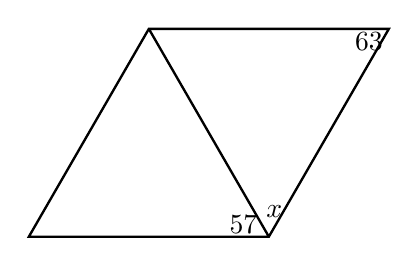
\begin{tikzpicture}

\def\len7{\lenB}

\draw[line width=0.3mm] (0,0) coordinate (a)  -- (0:0.8*\len7) coordinate (b) --++ (60:0.8*\len7) coordinate (c) -- (60:0.8*\len7) coordinate (d) -- cycle (b) -- (d) ;  

\node[anchor=south east, inner sep=1pt, rotate=0, xshift=-0.3em, yshift=0pt] (62-label) at (b) {$ 57\degree $}; 

\node[anchor=south, inner sep=1pt, rotate=0, xshift=0.2em, yshift=1.3ex] (x-label) at (b) {$ x\degree $}; 

\node[anchor=north east, inner sep=1pt, rotate=0, xshift=-0.1em, yshift=0pt] (c-label) at (c) {$ 63\degree $}; 

\end{tikzpicture} \\
\hline
6. 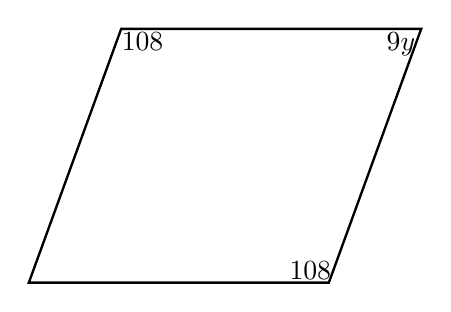
\begin{tikzpicture}

\def\len6{\lenB}

\draw[line width=0.3mm] (0,0) coordinate (a)  -- (0:\len6) coordinate (b) --++ (70:0.9*\len6) coordinate (c) -- (70:0.9*\len6) coordinate (d) -- cycle;  

\node[anchor=south east, inner sep=1pt, rotate=0, xshift=0.2em, yshift=0pt] (b-label) at (b) {$ 108\degree $}; 

\node[anchor=north west, inner sep=1pt, rotate=0, xshift=-0.1em, yshift=0pt] (d-label) at (d) {$ 108\degree $}; 

\node[anchor=north east, inner sep=1pt, rotate=0, xshift=-0.1em, yshift=0pt] (c-label) at (c) {$ 9y\degree $}; 

\end{tikzpicture} 
& 
8. 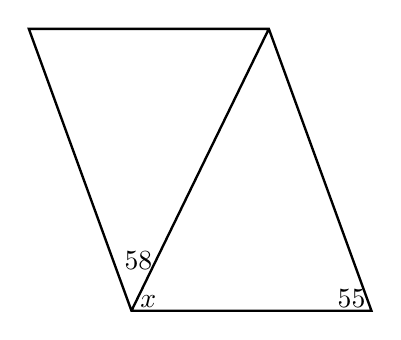
\begin{tikzpicture}

\def\len8{\lenB}

\draw[line width=0.3mm] (0,0) coordinate (a)  -- (0:0.8*\len8) coordinate (b) --++ (110:\len8) coordinate (c) -- (110:\len8) coordinate (d) -- cycle -- (c) ;  

\node[anchor=south east, inner sep=1pt, rotate=0, xshift=-0.1em, yshift=0pt] (b-label) at (b) {$ 55\degree $}; 

\node[anchor=south west, inner sep=1pt, rotate=0, xshift=0.2em, yshift=0pt] (x-label) at (a) {$ x\degree $}; 

\node[anchor=south, inner sep=1pt, rotate=0, xshift=0.25em, yshift=3.2ex] (58-label) at (a) {$ 58\degree $}; 

\end{tikzpicture} \\
\hline
\end{tabularx} 
\end{minipage}
\end{center} 
 